\section{Proposed Mamba-MCU Optimizations}
\label{sec:methodology}

This section details the deployment framework and architectural adaptations developed to enable efficient Mamba inference on microcontrollers. We outline our hardware and toolchain selection criteria, describe the custom model re-implementation pipeline, and introduce three targeted optimization strategies: hardware-aware activation simplification, post-training integer quantization, and a modular loop-partitioning scheme to mitigate compilation unrolling.

\subsection{Embedded Deployment Toolchain and Hardware Selection}
\label{sec:embedded_deployment}

Deploying state-space models on resource-constrained microcontrollers introduces significant engineering trade-offs. While MambaLite-Micro \cite{xuMambaLiteMicroMemoryOptimizedMamba2025} ensures that the output matches the PyTorch model output in 100\% of cases by hardcoding entire inference in C, this approach severely restricts flexibility. Any architectural modification or optimization like replacing activation functions or introducing quantization requires manual code modifications to the low-level source code, hindering rapid experimentation.

To overcome this limitation, this work establishes an automated, hardware-agnostic compilation pipeline. We evaluated contemporary edge runtime environments, including TensorFlow Lite for Microcontrollers (TFLM, recently being rebranded into LiteRT) \cite{davidTensorFlowLiteMicro2021} and ExecuTorch \cite{executorch2026}. TFLM was selected due to its mature ecosystem, robust documentation, and flexible runtime interpretation. By mapping operations directly to the TFLM runtime, this workflow eliminates intermediary conversion formats (e.g., ONNX), thereby isolating the experimental results from unnecessary intermediary model representations.

The deployment infrastructure leverages several utility tools embedded within the TFLM ecosystem. The compiler utility \texttt{tflm\_model\_transforms} strips redundant metadata and debugging nodes from the intermediate representation graph, isolating the raw architectural parameters and facilitating a rigorous, equitable comparison of binary model sizes. For precision reduction, we deploy the AI Edge Quantizer, which provides fine-grained, programmatic configuration over tensor bit-widths directly on the compiled flatbuffer files. The comprehensive deployment pipeline is structured as illustrated in \autoref{fig:deployment}.

\begin{figure}[ht]
  \centering
  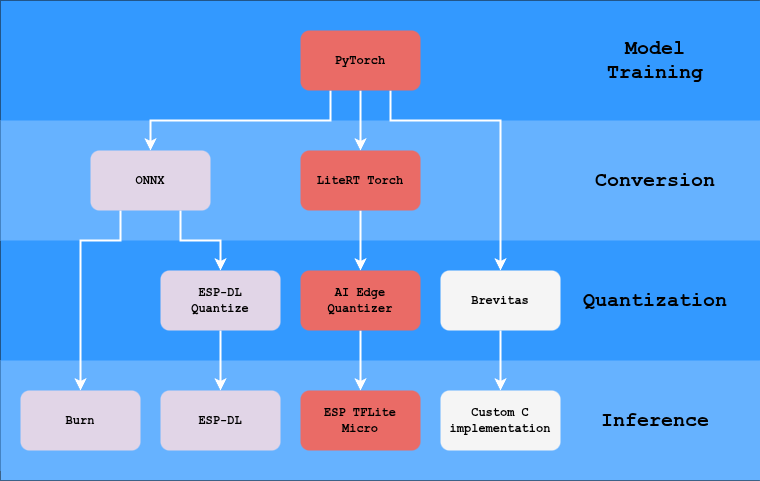
\includegraphics[width=\linewidth]{assets/deployment_diagram.drawio.png}
  \caption{Diagram of the TinyML deployment pipeline. The specific optimization path implemented in this work is highlighted in red.}
  \label{fig:deployment}
\end{figure}

Alternative model compression libraries were also considered, such as Brevitas \cite{brevitas} (leveraged in FEMBA \cite{tegonFEMBAEdgePhysiologicallyAware2026a}) and TorchAO \cite{orTorchAOPyTorchNativeTrainingtoServing2025}. While these frameworks provide robust support for Quantization-Aware Training (QAT) and ultra-low mixed-precision bit-widths, they frequently assume low-level kernel fusion capabilities. Such optimizations are challenging to synthesize efficiently on generic microcontrollers without specialized hardware abstractions.

Physical hardware evaluation is conducted on the Espressif ESP32 family of microcontrollers (\autoref{fig:esp32}), specifically the ESP32 and ESP32-S3 modules, using the vendor-optimized \texttt{esp-tflite-micro} component library. To ensure the generalizability of our findings across competing hardware platforms, we explicitly avoid vendor-exclusive deployment pipelines such as ESP-DL or STM32Cube.AI.

\begin{figure}[ht]
  \centering
  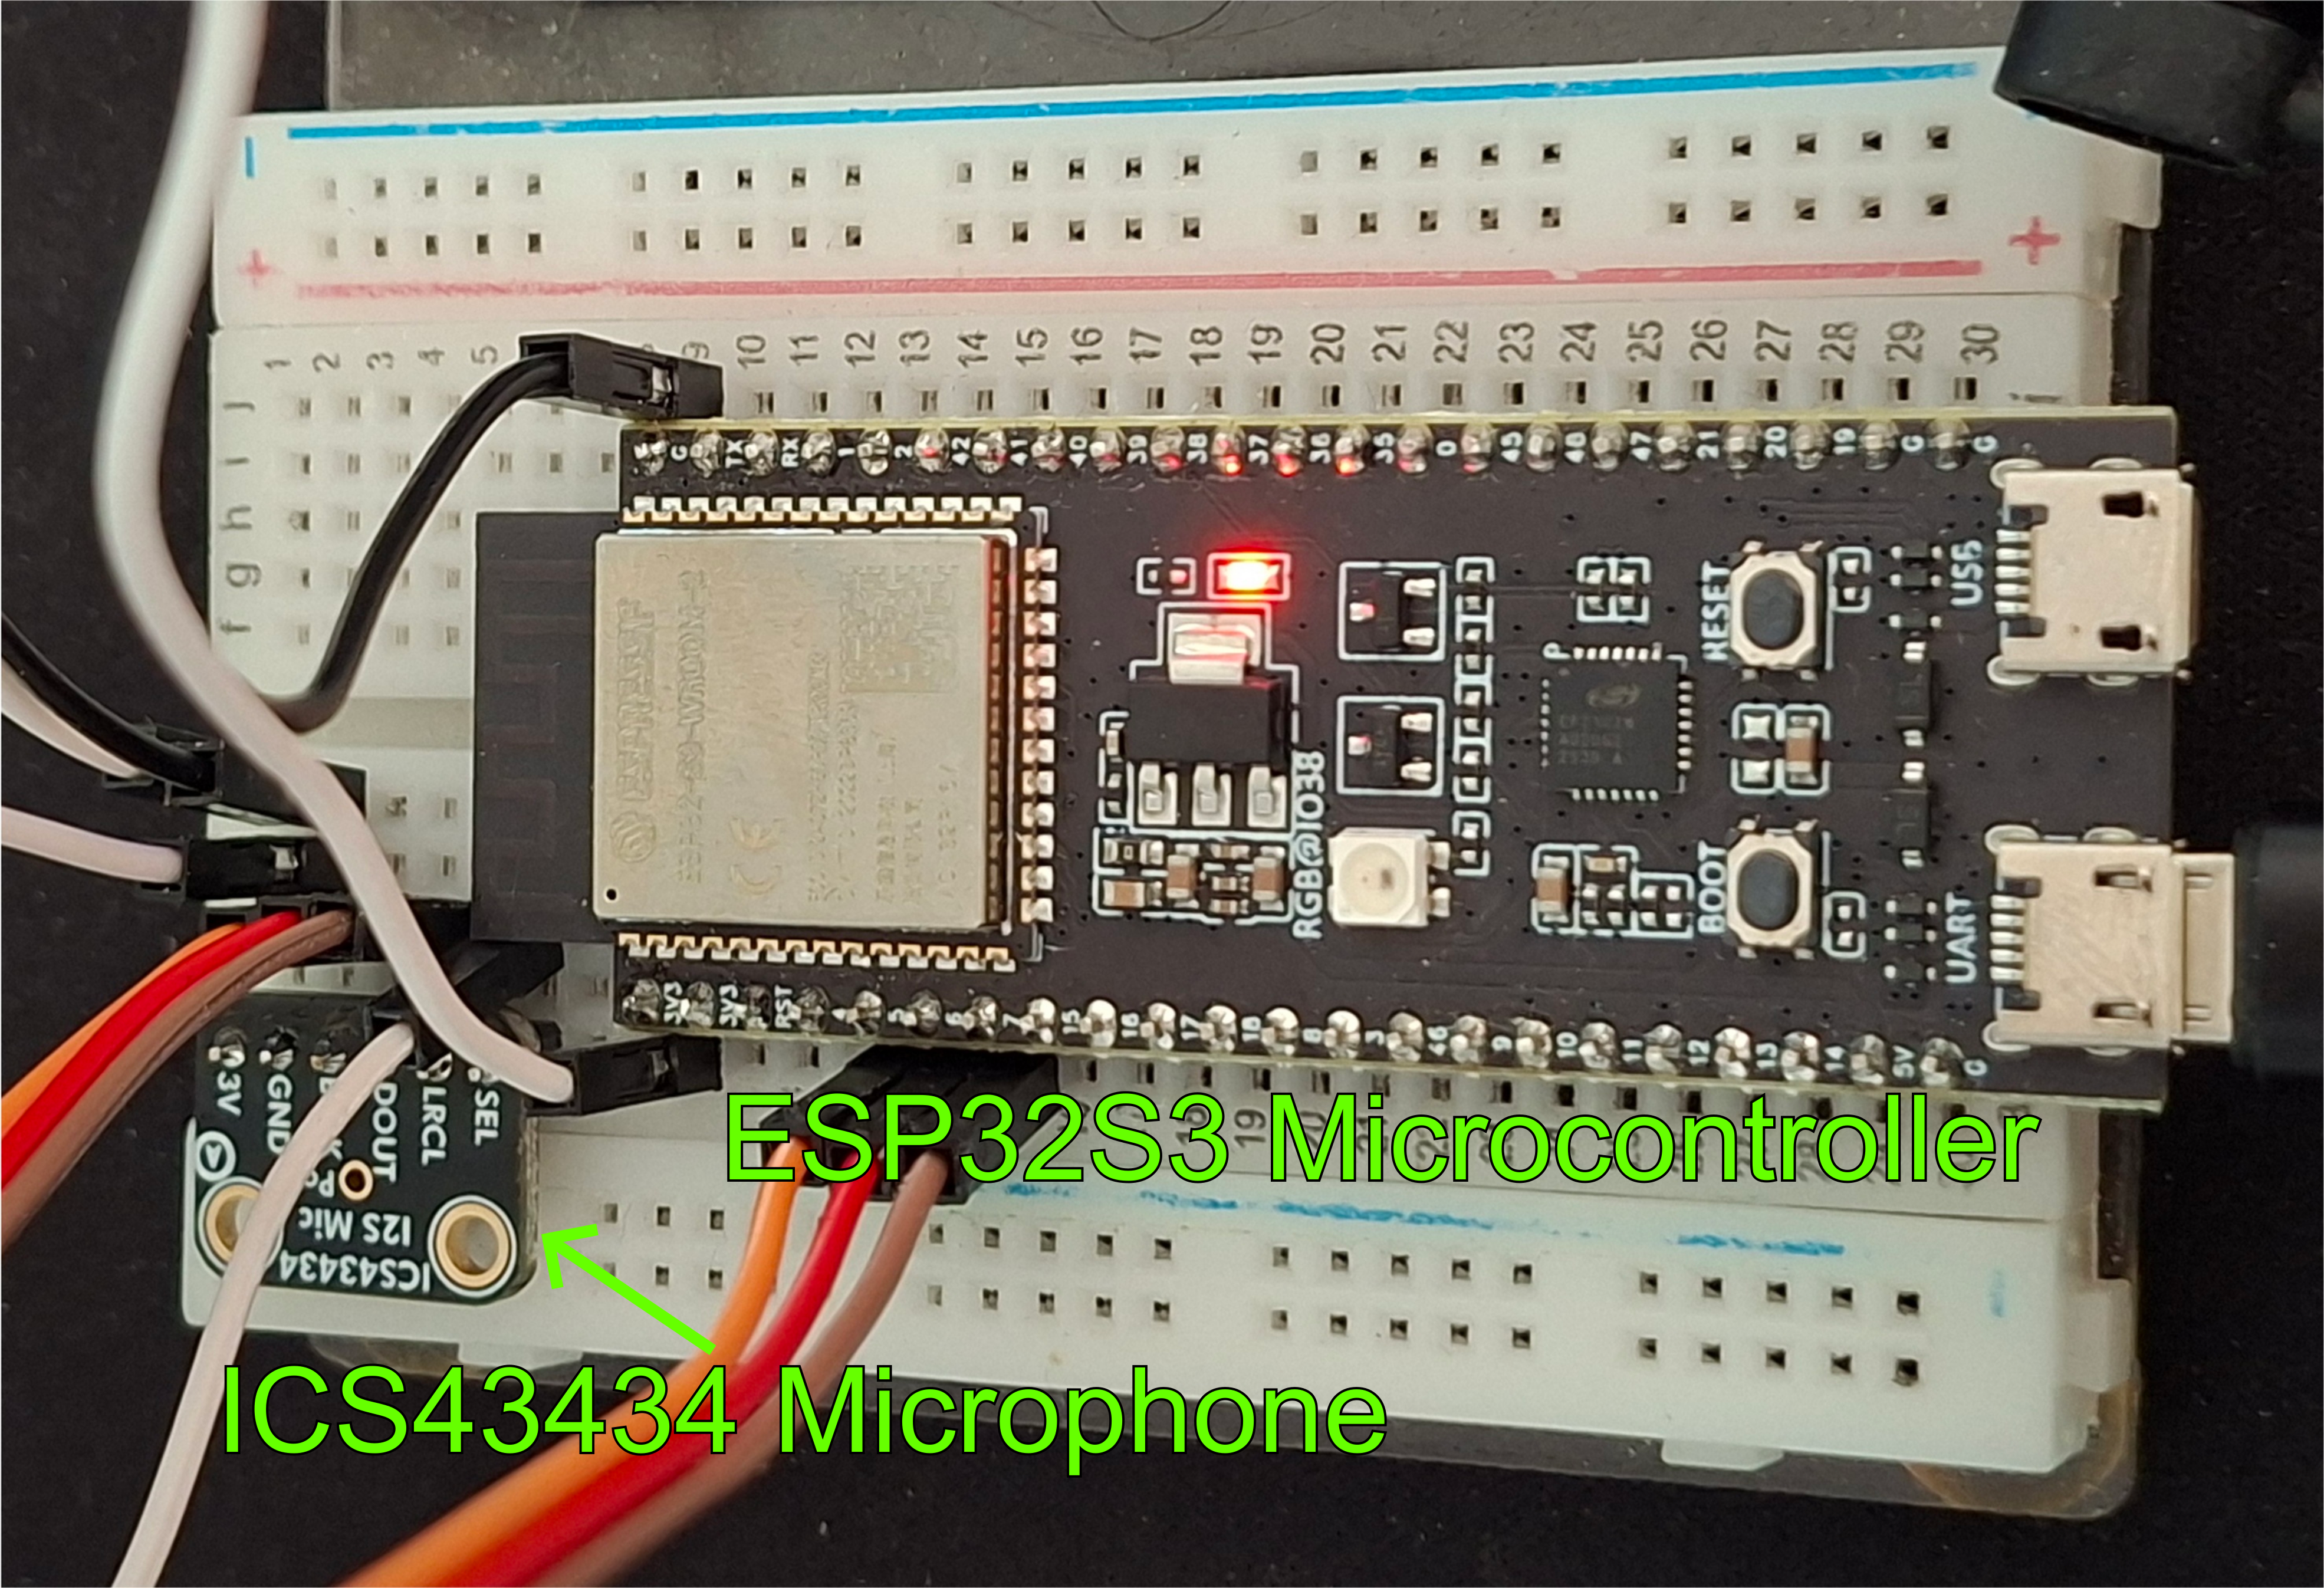
\includegraphics[width=0.7\linewidth]{assets/esp32.png}
  \caption{Experimental setup featuring an ESP32-S3 microcontroller coupled to an ICS43434 microphone module.}
  \label{fig:esp32}
\end{figure}

\subsection{System Design and Architectural Adaptations}

To maintain empirical continuity and isolate the performance impacts of our deployment optimizations, we adopt the core structural dimensions of the MambaLite-Micro baseline \cite{xuMambaLiteMicroMemoryOptimizedMamba2025} rather than performing an exhaustive hyperparameter grid search. The reference network consists of a fully connected projection layer, a single Mamba block ($d_{\text{model}} = 64$, expansion factor $E = 2$), a global average-pooling layer, and a linear output classification head.

Because standard Mamba implementations rely heavily on custom Triton or CUDA GPU kernels that lack native equivalents in edge runtimes, we re-implemented the network graph using standard, modular operators in PyTorch. This re-implementation provides malleable graph structures allowing us to swap mathematically intensive, exponentiation-heavy activation functions (e.g., SiLU) for hardware-friendly primitives (e.g., ReLU) prior to model compilation.

Following initial profiling cycles, the state-space formulation and transcendental activation layers emerged as the dominant latency and memory bottlenecks. In our work we focus on those two main issues, by simplifying the activation functions and suggesting a solution for the SSM layer.

Furthermore, initial deployment trials exposed a systemic limitation within the TFLM translation layer: the absence of native recurrent loop primitives caused the execution graph of the Selective State-Space Model to compile as a completely unrolled sequence. For long-context workloads, such as the Google Speech Commands V2 dataset, this unrolling behavior triggers an exponential explosion in model binary size and completely breaks execution due to constraints on the \texttt{CONCATENATE} operator nodes.

To resolve this sequence scaling ceiling, we introduce a modular loop-partitioning design pattern. The model is decoupled into three independent execution stages: pre-SSM projection phase, SSM time-step kernel, post-SSM output phase.

The host microcontroller code executes an explicit iterative loop around the single-step SSM kernel component, sequentially cycling through the inputs while maintaining the hidden state vector in native memory. This approach eliminates graph duplication by recycling a single set of network weights across all time steps. To quantify the execution trade-offs inherent to this approach, we bench-test both the unrolled and loop-partitioned implementations on the Human Activity Recognition (HAR) dataset \cite{anguitaPublicDomainDataset2013}. Notably, the unrolled baseline fails to run on the long-sequence Google Speech Commands V2 \cite{speechcommandsv2} workload because of the graph size (after 51 sequence step) unrolling being too large. This makes the loop-partitioned paradigm a strict architectural prerequisite for complex audio tasks.

\subsection{Showcase Demonstration: Keyword Spotting on ESP32-S3}

To demonstrate the practical viability of our proposed optimizations, we deploy a quantized Mamba model on an ESP32-S3 microcontroller for a Keyword Spotting task. The model is trained on the Google Speech Commands V2 dataset. It is built on top of the tensorflow micro speech example for efficient preprocessing. The audio gathering is done using an ICS43434 microphone module. Data gathering and inference runs fully on the microcontroller and it is able to process audio samples two times per second.
